\chapter{Introduction}

%%%%%%%%%%%%%%%%%%%%%%%%%%%%%%%%%%%%%%%%%%%%%%%%%%%%%%%%%%%%%%%%%%%%%%%%%%%%%%%%%%%%
% SECTION: Background to the study
%%%%%%%%%%%%%%%%%%%%%%%%%%%%%%%%%%%%%%%%%%%%%%%%%%%%%%%%%%%%%%%%%%%%%%%%%%%%%%%%%%%%
\section{Background to the study}

The human behavioural and anatomical activities are influenced by several internal cycles. Among them is the \textbf{circadian rhythm}, a rhythm studied for many years and whose impacts on the human activity has lead to new interests in the regulation of these activities. Formally defined as a \textit{"cyclical changes in hormones, body temperature, and other biological processes over the course of a 24 hour period"} \cite{ge2014}, the \textbf{Natural Institute of Health (NIH)} defines it as \textit{"a physical, mental and behavioural changes that follow a roughly 24-hour cycle, reponding primarily to light and darkness in an organism's environment"}\cite{ge2014}. The circadian rhythm plays an important role as its also affect the human sleeping and rising pattern. The circadian rhythm is influenced by the production of \textit{melatonin} produced by the \textit{pineal gland} whose activitties are dependent on the presence of light on the \textit{retinal-hypothalamic tract}\cite{lig1994}.These studies have shown that the presence of light with specifics wavelength at certain period of time during a day can affect the normal sleeping cycle.\\   
According to the NIH, there is a correlation between long-term health problems and and sleep disorders \cite{ph2002}. While stress levels and lifestyles affect the sleeping pattern, there is a strong evidence that light have a greater effect. With the invention of the electric light and the recent human exposure to LED screen, human have more exposure to light. Recent researches have shown that the usage of LED technologies at night is linked to sleep deficiency. Blueish light is said to have an huge impact on one of the human internal clock. Sleep deficiency due to inapropriate light exposure can be cured using an optimal light exposure. Researchers were able to quantify, qualify and time the light that is suitable to maintain the natural sleep-awake cycles \cite{cir2014}. With these results, it is possible to create an environment that will follow user specific light requirment needed to treat patient with sleep disorder.


%%%%%%%%%%%%%%%%%%%%%%%%%%%%%%%%%%%%%%%%%%%%%%%%%%%%%%%%%%%%%%%%%%%%%%%%%%%%%%%%%%%%
% SECTION: Objectives of this study
%%%%%%%%%%%%%%%%%%%%%%%%%%%%%%%%%%%%%%%%%%%%%%%%%%%%%%%%%%%%%%%%%%%%%%%%%%%%%%%%%%%%
\section{Objectives of this study}

\subsection{Problems to be investigated}
This project investigates the feasability of making user friendly embedded system, relatively cheap that could be used as a personal medical device in solving human sleep disorder.

\subsection{Purpose of the study}
The purpose of this study is to create a device that can be used to improve the user's sleeping pattern and to create a user friendly and personalisable digital alarm clock. The product would need to be relatively cheap and have more features than its competitor. Ideally, the NPSC would use medical lighting requirements and patterns for its users in order to be used an a prsonal medical device in the cure of sleeping disorder.  



%%%%%%%%%%%%%%%%%%%%%%%%%%%%%%%%%%%%%%%%%%%%%%%%%%%%%%%%%%%%%%%%%%%%%%%%%%%%%%%%%%%%
% SECTION: Scope and Limitations
%%%%%%%%%%%%%%%%%%%%%%%%%%%%%%%%%%%%%%%%%%%%%%%%%%%%%%%%%%%%%%%%%%%%%%%%%%%%%%%%%%%%
\section{Scope and limitations}

The scope of this project involves the design of an functional embedded system named \textbf{NeoPixels Sunrise Clock} aslo known as \textbf{NPSC}, capable of producing light of $460nm$ with an intensity of $30 lux$ as mentioned by the paper \textit{\textbf{"Action Spectrum for Melatonin Regulation in Humans: Evidence for a Novel Circadian Photoreceptor"}}. The code and design artefact repository and a full documentation including a user manual, for anybody who wants to make use of the code design resources, also need to the delivered. Moreover, a descripion of future use of the device in the study of the effect of light on the circadian rhythm will be required.\\
This project does not study the effect of light on the users. For ethical reasons, the NPSC will not be tested  on human subjects in real situations of either waking humans or including lighting to facilitate sleep at night. Instead the system will be tested based on the recommendation from the research  literature.\\
The design and creation of the NPSC is subject to several constraints listed below:
\begin{itemize}
\item \textbf{Time:} The project has a duration of 12 weeks within which the research, design, development, implementation, verification, and report writing need to be done.
\item \textbf{Money:} The project budget allocation is \textbf{R1000}
\item \textbf{Light:} The NPSC must be able able to produce blue light with wavelength of $460nm$ while providing enought light to meet the requirement of the research paper and provide a various range of colour for sunrise simulation. These requirements narrow the options for choosing the right light emmiters.
\item \textbf{Size:} The NPSC is meant to be a bedside lamp, this implies that it should have a relatively small size to be able to fit on a $50cm*50cm$ bedside table.
\end{itemize}


%%%%%%%%%%%%%%%%%%%%%%%%%%%%%%%%%%%%%%%%%%%%%%%%%%%%%%%%%%%%%%%%%%%%%%%%%%%%%%%%%%%%
% SECTION: Plan of Development
%%%%%%%%%%%%%%%%%%%%%%%%%%%%%%%%%%%%%%%%%%%%%%%%%%%%%%%%%%%%%%%%%%%%%%%%%%%%%%%%%%%%
\section{Plan of development}

The project was broken into sections and subsections with an estimated timeline.\\
The \textit{Gantt Chart} used for this project is shown in \cref{fig:gant}. The project started with the an intensive research on the science related to the human sleeping cycle. The research lead to the design of the NPSC consisting of its hardware and software modules. During the manufacturing process, the software framework of the NPSC was continously improved. The NPSC hardware and software integration were done later after the assembly of the hardware. Finally, the software was improved during the remaining lifetime of the project.
\begin{figure}[ht]
\centering
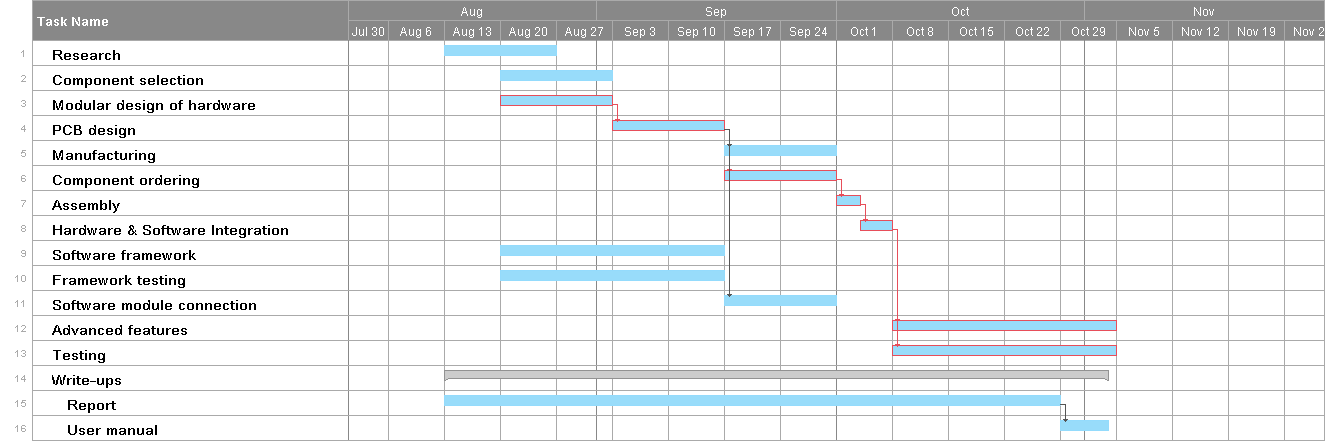
\includegraphics[scale=0.35]{gantt_chart.png}
\caption{Gantt chart showing the timeline of every task in the project as well as its critical path.}
\label{fig:gant}
\end{figure}

\begin{landscape}
\begin{figure}[ht]
\centering
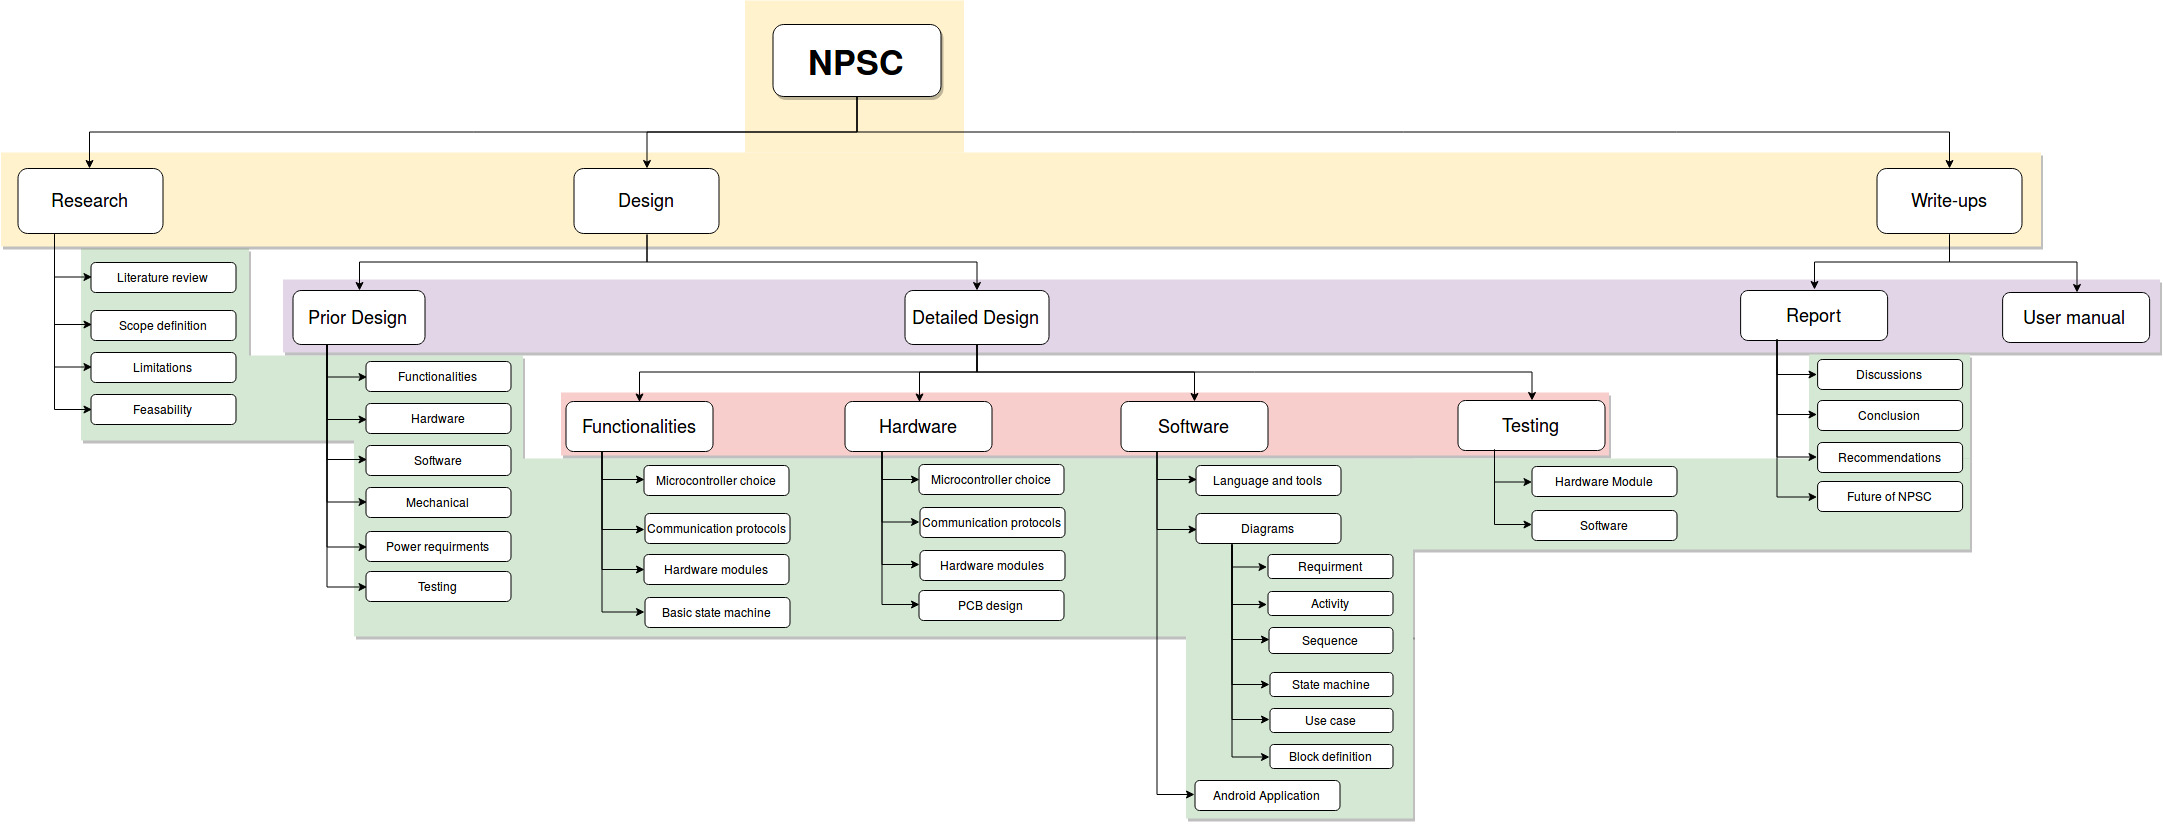
\includegraphics[scale=0.35]{wbs.jpg}
\caption{Report breakdown detailing the different sections needed to be included in the report.}
\label{fig:wbs}
\end{figure}
\end{landscape}

\subsection{Chronological progression of the report}
The report organisation is displayed in \cref{fig:wbs}. The sections of the report are explained below:
\begin{itemize}
\item \textbf{Research}
\begin{itemize}
\item \textbf{Introduction:} The feasability of the project as well as its scope and limitations are defined in the introduction. 
\item \textbf{Literature Review:} The literature review gives an insight in the researches made for this project. This includes scientific discoveries on the human sleeping cycle, experiements and results performed  by researchers on that matter, and some technical engineering design decisions. 
\end{itemize} 
\item \textbf{Design} 
\begin{itemize}
\item \textbf{Methodology:} This section covers the hardware, softeare, and mechanical design of the NPSC. 
\item \textbf{Results:} This section displays the results of the hardware and software testing. 
\end{itemize}
\item \textbf{Write-ups} 
\begin{itemize}
\item \textbf{Discussion:} The analysis of the results obtained. Here, the performance of the NPSC is evaluated. A costs and functional analysis of NPSC done to evaluate its performance compared to its competitors. Moreover, the future use of the NPSC is elaborated. 
\item \textbf{Conclusion:} An evaluation of the project, did we achieve the intended goals.
\item \textbf{Recommendations:} We dive into the solutions or recommendations that could improve the design of such device.
\item \textbf{User manual:} This section is for any users of the NPSC. It provides a clear explanation of the features of the NPSC and a detailed manual. 
\end{itemize}
\end{itemize}